% !TEX root = rapport.tex
% ============================================================
%  Cheebo — Final Year Project Report (PFE)
%  TEK-UP  |  Web, Mobile and Multimedia Development
%  Academic Year 2025-2026
% ============================================================
\documentclass[12pt, a4paper, oneside]{report}

% ── Encoding & language ─────────────────────────────────────
\usepackage[utf8]{inputenc}
\usepackage[T1]{fontenc}
\usepackage[english]{babel}

% ── Fonts ───────────────────────────────────────────────────
\usepackage{lmodern}

% ── Layout ──────────────────────────────────────────────────
\usepackage[
  top=2.5cm, bottom=2.5cm,
  left=3cm,  right=2.5cm
]{geometry}
\usepackage{setspace}
\onehalfspacing

% ── Graphics ────────────────────────────────────────────────
\usepackage{graphicx}
\usepackage{float}
\graphicspath{{images/}}          % put all images in ./images/

% ── Colors ──────────────────────────────────────────────────
\usepackage[dvipsnames]{xcolor}
\definecolor{cheeboblue}{RGB}{30, 64, 175}   % primary brand color
\definecolor{cheebolightgray}{RGB}{245, 245, 245}
\definecolor{sectiongray}{RGB}{80, 80, 80}

% ── Chapter / section style ──────────────────────────────────
\usepackage{titlesec}

% Chapter heading — bold, colored, with a rule
\titleformat{\chapter}[block]
  {\normalfont\LARGE\bfseries\color{cheeboblue}}
  {\chaptername~\thechapter}{1em}{}[{\titlerule[1pt]}]
\titlespacing*{\chapter}{0pt}{50pt}{20pt}

% Section
\titleformat{\section}
  {\normalfont\large\bfseries\color{cheeboblue}}
  {\thesection}{1em}{}
\titlespacing*{\section}{0pt}{18pt}{8pt}

% Subsection
\titleformat{\subsection}
  {\normalfont\normalsize\bfseries\color{sectiongray}}
  {\thesubsection}{1em}{}
\titlespacing*{\subsection}{0pt}{14pt}{6pt}

% ── Headers / footers ────────────────────────────────────────
\usepackage{fancyhdr}
\pagestyle{fancy}
\fancyhf{}
\fancyhead[L]{\small\textit{Cheebo}}
\fancyhead[R]{\small\textit{\nouppercase{\leftmark}}}
\fancyfoot[C]{\thepage}
\renewcommand{\headrulewidth}{0.4pt}
\setlength{\headheight}{16pt}
\setlength{\headsep}{28pt}
% Shorter chapter mark — no "Chapter N." prefix, just the title
\renewcommand{\chaptermark}[1]{\markboth{#1}{}}

% ── TOC style ────────────────────────────────────────────────
\usepackage{tocloft}
\renewcommand{\cftchapfont}{\bfseries\color{cheeboblue}}
\renewcommand{\cftsecfont}{\color{sectiongray}}
\setlength{\cftbeforechapskip}{6pt}

% ── Hyperlinks ───────────────────────────────────────────────
\usepackage[
  colorlinks=true,
  linkcolor=cheeboblue,
  urlcolor=cheeboblue,
  citecolor=cheeboblue,
  pdftitle={PFE Report — Cheebo},
  pdfauthor={Nadim Jebali},
]{hyperref}

% ── Listings (code) ──────────────────────────────────────────
\usepackage{listings}
\lstset{
  basicstyle=\ttfamily\small,
  backgroundcolor=\color{cheebolightgray},
  frame=single,
  breaklines=true,
  tabsize=2,
}

% ── Tables ───────────────────────────────────────────────────
\usepackage{booktabs}
\usepackage{tabularx}
\usepackage{array}
\usepackage{multirow}
\usepackage{longtable}
\usepackage{makecell}

% Centred X column for tabularx
\newcolumntype{C}{>{\centering\arraybackslash}X}

% MoSCoW priority colors
\definecolor{moscowMust}{RGB}{255, 182, 182}
\definecolor{moscowShould}{RGB}{255, 220, 150}
\definecolor{moscowCould}{RGB}{180, 210, 255}
\definecolor{moscowWont}{RGB}{220, 220, 220}
\definecolor{complexLow}{RGB}{180, 230, 180}
\definecolor{complexMed}{RGB}{255, 240, 150}
\definecolor{complexHigh}{RGB}{255, 200, 150}
\definecolor{complexVHigh}{RGB}{255, 170, 170}
% Feature group colors
\definecolor{featAuth}{RGB}{219, 234, 254}
\definecolor{featStore}{RGB}{220, 252, 231}
\definecolor{featProduct}{RGB}{204, 251, 241}
\definecolor{featOrder}{RGB}{254, 243, 199}
\definecolor{featAdmin}{RGB}{252, 231, 243}
\definecolor{featAI}{RGB}{237, 233, 254}
\definecolor{featPremium}{RGB}{254, 249, 195}
\definecolor{featCICD}{RGB}{224, 242, 254}
\definecolor{tableHeader}{RGB}{55, 65, 81}

\usepackage{colortbl}

% ── Misc ─────────────────────────────────────────────────────
\usepackage{enumitem}
\usepackage{caption}
\usepackage{subcaption}
\usepackage{pifont}       % checkmarks etc.
\usepackage{mdframed}     % info boxes

% Placeholder box (used wherever a real image is not yet available)
\newcommand{\imagePlaceholder}[2][8cm]{%
  \begin{mdframed}[backgroundcolor=cheebolightgray,linecolor=gray!40]
    \centering
    \vspace{#1}
    \textit{\color{gray}[IMAGE TO INSERT: #2]}
    \vspace{8mm}
  \end{mdframed}
}

% ── Opening environment for chapter intro paragraph ──────────
\newenvironment{chapterintro}{%
  \begin{mdframed}[backgroundcolor=cheebolightgray,linecolor=cheeboblue,linewidth=1pt]
  \small\itshape
}{%
  \end{mdframed}
}

% ── Key takeaways box (end of chapter) ───────────────────────
\newenvironment{keytakeaways}{%
  \par\bigskip
  \begin{mdframed}[
    backgroundcolor=cheebolightgray,
    linecolor=cheeboblue,
    linewidth=3pt,
    topline=false,
    bottomline=false,
    rightline=false,
    innerleftmargin=14pt,
    innerrightmargin=14pt,
    innertopmargin=10pt,
    innerbottommargin=10pt
  ]
  \noindent{\bfseries\color{cheeboblue}\large Key Takeaways}\par
  \vspace{4pt}
  \small
}{%
  \end{mdframed}
}

% ============================================================
\begin{document}

% ── Cover page ───────────────────────────────────────────────
\begin{titlepage}
  \centering
  \vspace*{0.5cm}

  % Header institutional block
  \textbf{Tunisian Republic}\\
  \textit{Ministry of Higher Education and Scientific Research}\\[4pt]
  \textbf{Private Higher School of Engineering and Technology}\\
  {\Large\textbf{TEK-UP}}

  \vspace{0.8cm}
  \rule{\textwidth}{1pt}
  \vspace{0.3cm}

  {\large Final Year Project Report}\\[4pt]
  \textit{Submitted in partial fulfilment of the requirements for the}\\
  \textbf{National Engineering Degree in Applied and Technological Sciences}\\
  \textit{Speciality: Web, Mobile and Multimedia Development}

  \vspace{0.5cm}
  \textit{Prepared by}\\[4pt]
  {\LARGE\textbf{Nadim JEBALI}}

  \vspace{0.8cm}
  % Logos: TEK-UP (left) and NeuralBey (right)
  \begin{figure}[H]
    \centering
    \begin{minipage}{0.45\textwidth}
      \centering
      
\includegraphics[height=2.5cm]{TEK-UP logo.png}
    \end{minipage}\hfill
    \begin{minipage}{0.45\textwidth}
      \centering
      
\includegraphics[height=2.5cm]{NeutalBey logo.jpeg}
    \end{minipage}
  \end{figure}

  \vspace{0.6cm}
  {\LARGE\bfseries\color{cheeboblue}
    Design and Development of an Intelligent\\
    Multi-Vendor Marketplace: Cheebo
  }

  \vspace{1cm}
  \begin{tabular}{rl}
    \textbf{Professional Supervisor:} & Mr. Mohammed Aziz Chibani \\
                                      & \textit{NeuralBey} \\[6pt]
    \textbf{Academic Supervisor:}     & Ms. Sawssen Jalel \\
                                      & \textit{Lecturer} \\
  \end{tabular}

  \vfill
  \rule{\textwidth}{1pt}\\[4pt]
  \textbf{Academic Year 2025 -- 2026}
\end{titlepage}

% ── Authorisation page ───────────────────────────────────────
\newpage
\thispagestyle{empty}
\vspace*{4cm}
\begin{center}
  \large
  I authorise the student to submit his internship report for a defence.\\[1.5cm]
  \textbf{Professional Supervisor, Mr. Mohammed Aziz Chibani}\\[0.4cm]
  \textit{Signature and stamp}\\[2cm]
  I authorise the student to submit his internship report for a defence.\\[1.5cm]
  \textbf{Academic Supervisor, Ms. Sawssen Jalel}\\[0.4cm]
  \textit{Signature}
\end{center}

% ── Dedication ───────────────────────────────────────────────
\newpage
\thispagestyle{empty}
\chapter*{Dedication}
\addcontentsline{toc}{chapter}{Dedication}

% Dedication

\vspace*{2cm}
\begin{center}
  \itshape
  To my parents, for their unwavering love, patience and encouragement during every step of this project.\\[1cm]
  To my friends and colleagues at NeuralBey and TEK-UP who offered guidance, feedback and inspiration.
\end{center}

% ── Acknowledgements ─────────────────────────────────────────
\newpage
\chapter*{Acknowledgements}
\addcontentsline{toc}{chapter}{Acknowledgements}

I would like to express my sincere gratitude to all those who contributed to the completion of this project.\\

First, my deepest thanks to my professional supervisor, Mr. Mohammed Aziz Chibani (NeuralBey), for his continuous guidance, domain expertise, and support throughout the development and evaluation phases.\\

I am also grateful to Ms. Sawssen Jalel for her academic supervision and valuable feedback which helped shape the report.\\

Special thanks to my colleagues and friends for testing features, providing constructive critiques, and motivating me during challenging moments.\\

Finally, I thank my family for their encouragement and patience during this work.

% ── Abstract ─────────────────────────────────────────────────
\newpage
\chapter*{Abstract}
\addcontentsline{toc}{chapter}{Abstract}

% TODO: English abstract (150-200 words)

\bigskip
\noindent\textbf{Keywords:} marketplace, multi-vendor, NestJS, React, Prisma,
  Artificial Intelligence, Docker, CI/CD, Terraform.

\bigskip\bigskip
\noindent\rule{\textwidth}{0.4pt}
\bigskip

% TODO: English abstract (150-200 words)

% ── Lists ────────────────────────────────────────────────────
\newpage
\tableofcontents

\newpage
\listoffigures

\newpage
\listoftables

% ── List of abbreviations ────────────────────────────────────
\newpage
\chapter*{List of Abbreviations}
\addcontentsline{toc}{chapter}{List of Abbreviations}

\begin{tabular}{ll}
  \textbf{AI}     & Artificial Intelligence \\
  \textbf{API}    & Application Programming Interface \\
  \textbf{CD}     & Continuous Deployment \\
  \textbf{CI}     & Continuous Integration \\
  \textbf{DB}     & Database \\
  \textbf{DNS}    & Domain Name System \\
  \textbf{DTO}    & Data Transfer Object \\
  \textbf{DWMM}   & Web, Mobile and Multimedia Development \\
  \textbf{JWT}    & JSON Web Token \\
  \textbf{ORM}    & Object-Relational Mapping \\
  \textbf{PFE}    & Final Year Project \\
  \textbf{REST}   & Representational State Transfer \\
  \textbf{SPA}    & Single Page Application \\
  \textbf{SSH}    & Secure Shell \\
  \textbf{UML}    & Unified Modeling Language \\
  \textbf{VPC}    & Virtual Private Cloud \\
\end{tabular}

% ============================================================
%  GENERAL INTRODUCTION
% ============================================================
\newpage
\chapter*{General Introduction}
\addcontentsline{toc}{chapter}{General Introduction}
\markboth{General Introduction}{}

This introduction explains the context for the Cheebo project, why the system was created, who the intended users are, and how the work was organised from conception through delivery.

Cheebo is a multi-vendor marketplace developed as a final year engineering project in partnership with TEK-UP and NeuralBey. The platform is designed to give Tunisian sellers a modern, secure online storefront while offering customers an intelligent shopping experience and administrators a reliable way to manage vendors, products, and verification workflows.

The project combines academic goals and real-world needs: it must satisfy the PFE requirements for software engineering, while also providing a practical solution that addresses the host organisation’s expectations for a modern web application. The following chapters present the host organisation, the business context, the requirements analysis, the system architecture, implementation details, and the deployment strategy.

% ============================================================
%  CHAPTER 1
% ============================================================
\chapter{General Project Context}

\begin{chapterintro}
  This chapter sets the scene --- why this project exists, who it is for,
  and how its development was organised. It introduces the host organisation,
  the business motivation behind Cheebo, the competitive landscape in which
  it operates, the proposed solution, and the working methodology adopted
  throughout the internship.
\end{chapterintro}

\section{Presentation of the Host Organisation}

\subsection{NeuralBey --- Company Overview}

NeuralBey is a Tunisian technology company that delivers end-to-end
engineering services across a broad spectrum of modern computing fields.
The company positions itself as a partner that translates client visions
into working systems, summarised by its own statement: \textit{``From web
and mobile apps to AI systems, IoT, embedded engineering, and 3D
solutions --- we build the technology that powers your vision.''}

This breadth allows NeuralBey to handle a project from initial concept
through deployment without external dependencies, and to combine
disciplines that are usually siloed --- for example, integrating
artificial intelligence into conventional web platforms, or interfacing
embedded devices with cloud services. The company's portfolio reflects
this versatility:

\begin{itemize}[leftmargin=*,itemsep=2pt]
  \item \textbf{Web and mobile applications} for consumer products and
        enterprise tooling;
  \item \textbf{AI systems}, including model integration, automation
        pipelines and intelligent assistants;
  \item \textbf{IoT and embedded engineering}, where NeuralBey designs
        firmware and connected devices;
  \item \textbf{3D solutions} for product visualisation, AR/VR and
        digital twins.
\end{itemize}

\subsection{Domain, Team and Mission}

NeuralBey operates as a multidisciplinary studio. Each project is
staffed by engineers selected from the relevant domain (frontend,
backend, AI, hardware, 3D), and a professional supervisor accompanies
the work from scoping through delivery. The team's working culture
emphasises code review, iterative delivery and frequent stakeholder
feedback --- practices that aligned naturally with the academic
requirements of a final year project.

The present project was carried out under the professional supervision
of \textbf{Mr.\ Mohammed Aziz Chibani}, who provided architectural
guidance, regular reviews, and technology recommendations throughout
the internship. Academic oversight was provided in parallel by
\textbf{Ms.\ Sawssen Jalel}, ensuring the work also satisfied the
methodological and documentation standards of the engineering diploma.

\section{Project Context}

\subsection{Project Origin and Motivation}

The Cheebo project originated from an internal need identified at
NeuralBey: the Tunisian online retail landscape lacks a modern,
multi-vendor platform that is both seller-friendly and equipped with
the automation features expected of contemporary marketplaces.
Existing local solutions are typically single-vendor stores or
classified-ad sites, and they offer limited tooling for moderation,
content quality and discovery.

NeuralBey saw an opportunity for a product combining three
differentiating capabilities:

\begin{enumerate}[label=(\roman*),leftmargin=*,itemsep=2pt]
  \item a true multi-vendor model with self-service onboarding for
        sellers;
  \item AI-assisted moderation of stores and products to reduce
        manual review load;
  \item a deployment story that demonstrates contemporary DevOps
        practices end-to-end.
\end{enumerate}

The PFE topic was therefore scoped jointly with the professional
supervisor, with the explicit goal of producing a system that could
serve both as a portfolio piece for the company and as a foundation
for further internal development beyond the internship.

\subsection{Multi-Vendor Marketplace Concept}

A \emph{multi-vendor marketplace} is a platform on which independent
sellers operate their own stores within a shared environment governed
by a central operator. It differs from two adjacent models:

\begin{itemize}[leftmargin=*,itemsep=2pt]
  \item a \textbf{single-vendor store}, where the platform itself owns
        the inventory and the brand;
  \item a \textbf{classified-ad site}, where the platform only lists
        offers and plays no role in transactions or quality control.
\end{itemize}

A marketplace must reconcile three concerns simultaneously:
\textbf{seller autonomy} (each seller manages catalogue, branding and
inventory), \textbf{buyer trust} (the platform guarantees a baseline
of product authenticity and fulfilment) and \textbf{operator
governance} (administrators onboard sellers, moderate content, suspend
stores and curate featured selections). These three perspectives drive
the architecture of Cheebo: every feature is designed to balance
autonomy for sellers, trust for buyers, and control for administrators.
The integration of AI verification is a direct response to the
buyer-trust requirement at the scale a marketplace demands.

\subsection{Target Users}

Three actor categories were identified at the scoping stage:

\begin{itemize}[leftmargin=*,itemsep=4pt]
  \item \textbf{Customer} --- an end-user who browses the catalogue,
        places orders and tracks deliveries. Expects a fast,
        mobile-friendly experience with reliable search and clear
        product information.
  \item \textbf{Seller} --- a small or medium merchant who creates a
        store, manages a product catalogue and fulfils orders.
        Expects low onboarding friction, clear analytics, and
        protection against unfair competition from low-quality
        listings.
  \item \textbf{Administrator} --- the platform operator (NeuralBey
        staff) who reviews seller applications, moderates flagged
        content, curates featured stores, and intervenes when a store
        violates the marketplace rules.
\end{itemize}

\section{Study of Existing Solutions}

\subsection{Existing Tunisian E-Commerce Platforms}

Three categories of competing platforms were studied:

\begin{itemize}[leftmargin=*,itemsep=4pt]
  \item \textbf{Pan-African marketplaces (Jumia).} Jumia Tunisia is
        the most visible regional marketplace. It supports multiple
        vendors at scale and offers a polished customer experience,
        but seller onboarding is heavyweight and the platform is not
        tailored to small Tunisian merchants.
  \item \textbf{Classified-ad sites (Tayara, Affariyet).} Tayara
        dominates the local classified-ad market. It offers excellent
        discovery for sellers, but performs no escrow, no order
        management, no integrated payment and no quality moderation.
  \item \textbf{Single-vendor stores (MyTek, Wiki, etc.).} These are
        vertically integrated retailers that operate their own
        catalogue. They cannot be used by independent sellers.
\end{itemize}

\subsection{Limitations of Current Solutions}

From the study above, four gaps emerged:

\begin{enumerate}[label=\textbf{L\arabic*.},leftmargin=*,itemsep=2pt]
  \item \textbf{No AI-assisted moderation.} On existing platforms,
        store and product verification are entirely manual --- slow,
        inconsistent, and impractical at scale.
  \item \textbf{Heavyweight seller onboarding.} Pan-regional players
        require contractual paperwork unsuitable for small merchants.
  \item \textbf{Limited operator tooling.} Classified-ad sites have
        weak admin dashboards; single-vendor stores have none for
        external sellers.
  \item \textbf{Outdated technical foundations.} Several platforms
        still rely on monolithic stacks without modern CI/CD or
        infrastructure-as-code, making evolution costly.
\end{enumerate}

\subsection{Competitive Analysis}

Table~\ref{tab:competitors} summarises the comparison along the four
criteria that drove the design of Cheebo. A check mark (\ding{51})
indicates the criterion is fully supported, a cross (\ding{55})
indicates it is absent, and a tilde (\(\sim\)) indicates partial
support.

\begin{table}[H]
  \centering
  \caption{Comparative analysis of competing platforms}
  \begin{tabularx}{\textwidth}{lCCC}
    \toprule
    \textbf{Criterion}     & \textbf{Jumia} & \textbf{Tayara} & \textbf{Cheebo} \\
    \midrule
    Multi-vendor model     & \ding{51} & \(\sim\)  & \ding{51} \\
    AI verification        & \ding{55} & \ding{55} & \ding{51} \\
    Admin dashboard        & \(\sim\)  & \ding{55} & \ding{51} \\
    CI/CD pipeline (open)  & \ding{55} & \ding{55} & \ding{51} \\
    Lightweight onboarding & \ding{55} & \ding{51} & \ding{51} \\
    \bottomrule
  \end{tabularx}
  \label{tab:competitors}
\end{table}

\noindent The \texttt{C} column type used above is defined locally as a
centred variant of \texttt{X}; it is declared once in the preamble.

\section{Proposed Solution}

\subsection{Cheebo Overview}

Cheebo is a multi-vendor marketplace designed around three pillars:
a self-service seller experience, AI-assisted content verification,
and a modern, fully containerised deployment. The platform is built
as a single-page \textbf{React 19} application backed by a modular
\textbf{NestJS} API, with \textbf{MariaDB} as the relational store
and \textbf{n8n} acting as an orchestration layer for AI tasks.
Authentication is handled by \textbf{Better-Auth} with email
verification, and \textbf{Prisma} is used as the ORM. The full system
is packaged with Docker Compose, provisioned on DigitalOcean via
Terraform, and delivered through a GitHub Actions CI/CD pipeline.

Sellers create a store in minutes, populate it with products and
tags, and benefit from automatic AI verification that surfaces a
trust badge to potential buyers. Administrators review borderline
cases through a dedicated dashboard, suspend stores when needed, and
override automated decisions. Customers browse a unified catalogue,
place orders across multiple sellers in a single checkout, and
interact with an in-app AI assistant for discovery and support.

\subsection{Key Differentiators}

Five differentiators set Cheebo apart from the platforms surveyed in
the previous section:

\begin{enumerate}[label=\textbf{D\arabic*.},leftmargin=*,itemsep=2pt]
  \item \textbf{AI verification of stores and products} via an n8n
        workflow that calls a hosted LLM and writes back an
        \texttt{adminReviewed} flag plus a textual rationale.
  \item \textbf{Lightweight seller onboarding} through a seller
        application form reviewed by administrators, with a free tier
        offering a single store at zero cost.
  \item \textbf{Integrated administration tooling} (review, suspend,
        curate, cascade-delete) implemented as first-class features
        rather than database admin scripts.
  \item \textbf{Conversational data access} via a database-aware
        chatbot built on n8n, allowing administrators to query the
        platform in natural language.
  \item \textbf{Modern DevOps foundations} --- pnpm monorepo, Docker
        Compose, Terraform on DigitalOcean, and GitHub Actions
        CI/CD --- demonstrating production-grade engineering
        practices end-to-end.
\end{enumerate}

\subsection{Project Scope}

The scope was agreed with the professional supervisor and is split
between in-scope and out-of-scope items so that the deliverables
remain clear and bounded.

\noindent\textbf{In scope:} account creation and email verification;
seller application workflow with admin review; store and product
CRUD with image upload; tag-based product recommendations with a
top-seller fallback; order placement, items and history; admin
moderation panels (store suspension, cascade-delete); AI verification and chat assistant via n8n;
store-wide percentage sales with automatic badge propagation across products and search results;
AI-assisted storefront redesign via an n8n/Groq workflow;
premium tier unlocking additional stores; and infrastructure-as-code
deployment.

\medskip
\noindent\textbf{Out of scope} (deferred to future iterations):
integrated payment processing (e.g.\ Konnect or Stripe); a native
mobile application; advanced fraud detection; on-premise LLM
hosting; multi-currency support; and a full-text search engine such
as Elasticsearch or Typesense.

\section{Work Methodology}

\subsection{Classical vs Agile Approaches}

Every software project requires a methodological framework to organise
work, manage priorities, and guarantee the delivery of a quality
product. Two major families of methods have historically competed: the
\textbf{classical} (predictive) approach and the \textbf{agile}
(adaptive) approach. Their fundamental difference lies in how they
handle change and value delivery.

\medskip
\noindent\textbf{Classical approach --- Waterfall.}
The Waterfall method divides the project into strictly sequential
phases: requirements, design, development, testing, and delivery.
Each phase must be fully validated before the next begins. This model
suits projects whose requirements are stable and known in advance, but
it shows its limits as soon as the context evolves:

\begin{itemize}[leftmargin=*,itemsep=2pt]
  \item Requirements are frozen at launch; any late change is costly.
  \item The client sees a working product only at the very end of the project.
  \item Defects and risks are detected in the test phase, too late to
        address without significant impact.
  \item Documentation tends to be voluminous and quickly out of sync
        with the actual code.
\end{itemize}

\medskip
\noindent\textbf{Agile approach --- Core principles.}
Agility was born from the \textit{Agile Manifesto} (2001), which
champions collaboration, adaptability, and the continuous delivery of
value. Rather than planning the entire project upfront, work is
organised into \textbf{short cycles called sprints} (one to four
weeks), each producing a functional and tested increment. This
approach offers several concrete advantages:

\begin{itemize}[leftmargin=*,itemsep=2pt]
  \item Requirements are refined continuously from client and
        stakeholder feedback.
  \item Value is delivered from the first sprints; the product is
        usable well before the end of the project.
  \item Risks are identified and addressed early.
  \item Daily communication fosters responsiveness and team alignment.
\end{itemize}

\subsection{Why Scrum?}

Among the agile methodologies available --- Scrum, Kanban, XP,
SAFe --- \textbf{Scrum} was chosen to manage this project for the
following reasons:

\begin{itemize}[leftmargin=*,itemsep=4pt]
  \item \textbf{Flexibility:} the requirements of Cheebo evolved
        throughout the internship; Scrum allows supervisor feedback to
        be integrated at each sprint.
  \item \textbf{Visibility:} a prioritised backlog and bounded sprints
        provide a clear view of progress at any point.
  \item \textbf{Regular rhythm:} two-week sprints impose a structuring
        cadence well-suited to the internship calendar.
  \item \textbf{Frequent deliveries:} each sprint produces a
        functional increment, facilitating demonstrations and
        validations with the professional supervisor.
  \item \textbf{Industry adoption:} Scrum is the most widely practised
        agile framework, and its use in a PFE context prepares the
        student for professional practice.
\end{itemize}

\subsection{The Scrum Framework}

Scrum is an agile project management framework that helps teams
organise and supervise their work through values, principles, and
practices. It encourages teams to learn from experience, self-organise
while working on a problem, and reflect on their successes and
failures to continuously improve.

Figure~\ref{fig:scrum} illustrates the Scrum process: successive
sprints feed functional increments into the product, validated at
each iteration by the Product Owner.

\begin{figure}[H]
  \centering
  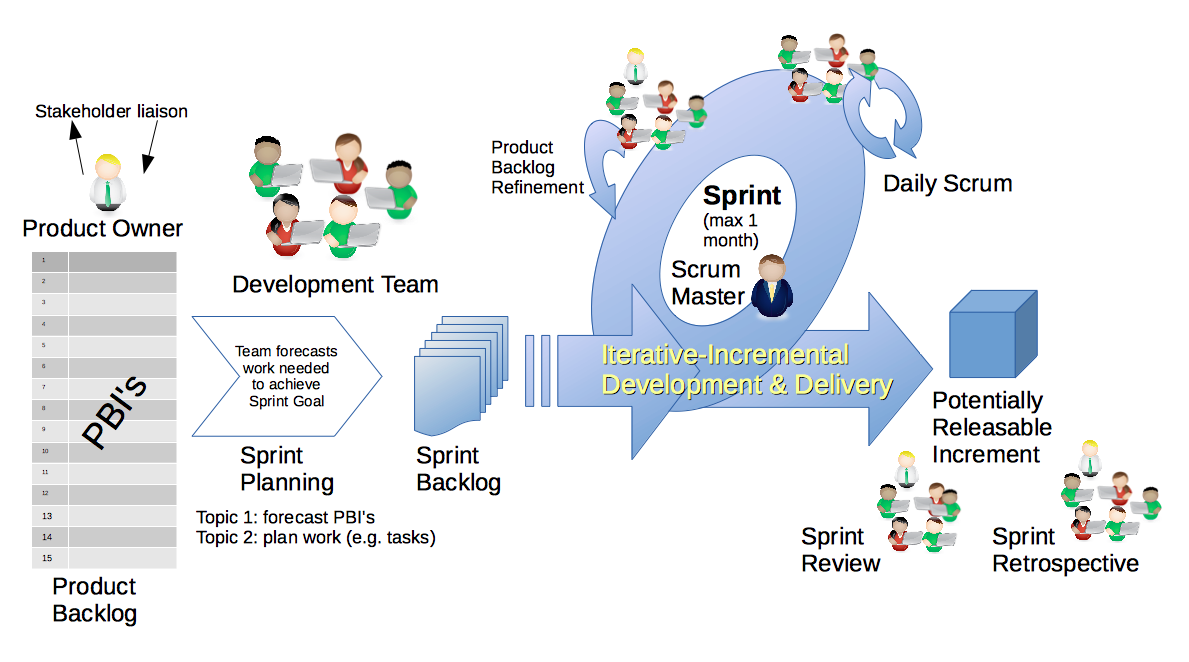
\includegraphics[width=0.85\textwidth]{scrum-framework.png}
  \caption[Scrum methodological framework]{Scrum methodological framework
    (source: Dr Ian Mitchell, Wikimedia Commons, CC0~/~CC~BY-SA~4.0).}
  \label{fig:scrum}
\end{figure}

\subsection{Scrum Roles}

Scrum defines three complementary roles:

\begin{itemize}[leftmargin=*,itemsep=4pt]
  \item \textbf{Product Owner:} represents the stakeholders and defines
        the product vision. He prioritises the Product Backlog items
        and validates each delivered increment. In this project, this
        role was fulfilled by \textbf{Mr.\ Mohammed Aziz Chibani}
        (NeuralBey), who approved the sprint backlog and conducted
        sprint reviews.
  \item \textbf{Scrum Master:} guarantees the application of the Scrum
        framework, facilitates team work, and removes obstacles. Given
        the single-developer nature of this PFE, this role was also
        assumed by Mr.\ Chibani, who provided architectural guidance
        and methodology coaching.
  \item \textbf{Development Team:} responsible for the technical
        realisation of features and the delivery of a potentially
        deployable increment at the end of each sprint. Composed in
        this project of the student, \textbf{Nadim Jebali}.
\end{itemize}

\subsection{Scrum Events}

The Scrum framework organises work around five key events:

\begin{itemize}[leftmargin=*,itemsep=4pt]
  \item \textbf{Sprint:} a fixed-duration iteration (two weeks in this
        project) during which the team produces a product increment.
  \item \textbf{Sprint Planning:} an opening meeting in which the team
        selects and plans the backlog items to realise during the
        sprint.
  \item \textbf{Daily Scrum:} a brief daily synchronisation of 15
        minutes to coordinate work and surface blockers.
  \item \textbf{Sprint Review:} a demonstration of the increment to
        stakeholders at the end of the sprint to collect feedback and
        validate progress.
  \item \textbf{Sprint Retrospective:} a process improvement meeting
        at the end of each sprint. Key improvements that emerged from
        retrospectives in this project include the adoption of
        \texttt{pnpm} for monorepo management, the migration from
        manual deployments to GitHub Actions, and the introduction of
        n8n for AI workflows.
\end{itemize}

\subsection{Scrum Artefacts}

Three artefacts ensure transparency of the work:

\begin{itemize}[leftmargin=*,itemsep=4pt]
  \item \textbf{Product Backlog:} a prioritised list of all expected
        product functionalities, maintained as user stories with
        MoSCoW priorities and complexity estimates (see
        Chapter~\ref{chap:requirements}).
  \item \textbf{Sprint Backlog:} a sub-set of the Product Backlog
        selected for a given sprint, broken down into technical tasks.
  \item \textbf{Increment:} a potentially deliverable version of the
        product obtained at the end of each sprint. The full project
        ran across approximately ten sprints, grouped into three
        milestones:
\end{itemize}

\begin{itemize}[leftmargin=*,itemsep=4pt]
  \item \textbf{Foundations (sprints 1--3):} repository setup,
        authentication with Better-Auth, base data model, and the
        seller-application flow.
  \item \textbf{Core marketplace (sprints 4--7):} stores, products,
        orders, admin panels, and tag-based recommendations.
  \item \textbf{Intelligence and delivery (sprints 8--10):} the AI
        verification pipeline, the in-app AI chat assistant,
        Dockerisation, Terraform provisioning, and the CI/CD
        pipeline.
\end{itemize}

\subsection{Tools Used}

The following tools were used throughout the project, covering source
control, development, containerisation, infrastructure provisioning,
workflow automation, and API testing.

% ── Tool card helper ─────────────────────────────────────────────────────────
% \toolcard{logo-file}{Tool Name}{Description}{Source URL}
\newcommand{\toolcard}[4]{%
  \begin{minipage}[t]{0.46\textwidth}
    \vspace{4pt}
    \begin{flushleft}
      \includegraphics[width=1.2cm,height=1.2cm,keepaspectratio]{images/#1}%
      \hspace{8pt}%
      \begin{minipage}[b]{0.78\linewidth}
        \textbf{\large #2}\\[2pt]
        {\small\url{#4}}
      \end{minipage}
    \end{flushleft}
    \vspace{4pt}
    \small #3
    \vspace{8pt}
    \hrule height 0.4pt
    \vspace{6pt}
  \end{minipage}%
}

\noindent
\toolcard{github.png}{GitHub}
  {A web-based platform for version control and collaborative software development
   built on Git. It was used for source control, code review via pull requests, and
   continuous integration and deployment through GitHub Actions workflows.}
  {github.com}
\hfill
\toolcard{notion.png}{Notion}
  {An all-in-one productivity workspace combining notes, databases, and kanban boards.
   It served as the project's backlog management tool, sprint board, and a living record
   of user stories and acceptance criteria.}
  {notion.so}

\noindent
\toolcard{vscode.png}{Visual Studio Code}
  {A lightweight but powerful source-code editor developed by Microsoft. It was the
   primary IDE throughout the project, extended with plugins for TypeScript, Prisma
   schema editing, ESLint linting, and Git integration.}
  {code.visualstudio.com}
\hfill
\toolcard{docker.png}{Docker}
  {An open platform for developing, shipping, and running applications inside isolated
   containers. It was used to containerise all services — PostgreSQL, the NestJS backend,
   the React frontend, and the n8n workflow engine — ensuring parity between development
   and production environments.}
  {docker.com}

\noindent
\toolcard{terraform.png}{Terraform}
  {An open-source infrastructure-as-code tool by HashiCorp that allows cloud resources
   to be defined in declarative configuration files. It was used to provision and manage
   the DigitalOcean droplet, DNS records, and firewall rules in a reproducible way.}
  {terraform.io}
\hfill
\toolcard{n8n.png}{n8n}
  {A fair-code workflow automation platform with a visual node-based editor. It was
   used to orchestrate the AI-assisted product and store verification pipeline as well
   as the in-app AI chat assistant, connecting the backend to large language model APIs.}
  {n8n.io}

\noindent
\toolcard{postman.png}{Postman}
  {A collaborative API development platform for designing, testing, and documenting
   HTTP endpoints. It was used during backend development to manually exercise and
   validate every REST endpoint before integration with the frontend.}
  {postman.com}
\hfill
\toolcard{pnpm.png}{pnpm}
  {A fast, disk-efficient package manager for Node.js that uses hard links and a
   content-addressable store. It managed all JavaScript dependencies across the
   monorepo workspace, ensuring consistent installs in both development and CI.}
  {pnpm.io}

\begin{keytakeaways}
\begin{itemize}[leftmargin=*,itemsep=2pt]
  \item Cheebo originates from an internal NeuralBey brief: build a
        modern, Tunisia-oriented multi-vendor marketplace with
        AI-assisted moderation.
  \item Three actors --- customer, seller, administrator --- drive
        every architectural decision throughout the report.
  \item Compared with Jumia and Tayara, Cheebo differentiates on
        \emph{AI verification}, \emph{lightweight seller onboarding},
        \emph{first-class admin tooling}, and \emph{modern DevOps}
        (Docker, Terraform, GitHub Actions).
  \item Development followed two-week Scrum sprints with NeuralBey
        reviews, structured around three milestones: foundations,
        core marketplace, and intelligence-and-delivery.
\end{itemize}
\end{keytakeaways}

\section*{Chapter Conclusion}
\addcontentsline{toc}{section}{Chapter Conclusion}

This chapter established the foundations of the Cheebo project. It
introduced NeuralBey, the host organisation, and explained the
business motivation behind building a modern Tunisian multi-vendor
marketplace. A study of existing platforms revealed four gaps ---
absent AI moderation, heavyweight onboarding, weak admin tooling, and
outdated technical foundations --- that Cheebo directly addresses.
The proposed solution, its key differentiators, and its bounded scope
were presented. Finally, the Scrum agile methodology was described
in detail, including its roles, events, and artefacts, and the
three-milestone sprint plan that organised the ten-week development
was outlined. The following chapter formalises the requirements
derived from this context.

% ============================================================
%  CHAPTER 2
% ============================================================
\chapter{Requirements Analysis and Specification}
\label{chap:requirements}

\begin{chapterintro}
  This chapter identifies the three system actors, formalises the
  functional and non-functional requirements of Cheebo, and illustrates
  them with UML use-case and sequence diagrams. The requirements were
  consolidated during the first three sprints in collaboration with the
  professional supervisor and serve as the contract that the rest of
  the report builds upon.
\end{chapterintro}

\section{Identification of Actors}

The platform recognises three actor categories. They are distinct
\textit{roles} stored on the \texttt{User} table rather than
distinct user records --- a single account can be promoted from
\textit{customer} to \textit{seller} once a seller application is
approved, and an administrator account is created automatically on
first boot.

\subsection{Customer}

The Customer is the default role assigned upon registration. A
Customer can browse the catalogue, search products, view individual
stores, manage a cart, place an order across multiple sellers in a
single checkout, and review their personal order history. The
Customer is also the entry point for the seller pipeline: any
Customer can submit a seller application and, once approved, gain
the Seller role on the same account. Anonymous (non-authenticated)
visitors share the read-only abilities of the Customer but cannot
maintain a cart or place an order.

\subsection{Seller}

The Seller is a Customer whose seller application has been approved
by an administrator. A Seller can create and edit one store under
the free tier (or several under the premium tier), populate that
store with products, upload product images, attach product tags,
view per-store analytics, and consult the order history specific to
their store. Sellers also choose a visual template for their store
from the templates exposed by the frontend. They cannot, however,
review or moderate the work of other sellers.

\subsection{Administrator}

The Administrator is created automatically by the backend at first
boot and is not exposed through the registration form. The
Administrator reviews seller applications, browses every store and
every product on the platform, suspends or deletes stores (with
cascading deletion of dependent records), overrides automated AI
verification decisions, curates featured stores and products on the
landing page, manages categories and sub-categories, and consults
the platform through a database-aware AI chat assistant.

\section{Functional Requirements}

The functional requirements are grouped into seven domains. Each
domain corresponds to a NestJS module on the backend and to a
matching set of pages on the React frontend; the mapping is made
explicit in Chapter~3.

\subsection{User Registration and Authentication}

\begin{enumerate}[label=\textbf{FR-A\arabic*.},leftmargin=*,itemsep=2pt]
  \item The system shall allow a visitor to create an account with
        an email address and password.
  \item The system shall send a verification email containing a
        one-time link upon successful registration.
  \item The system shall prevent unverified accounts from creating a
        store or placing an order.
  \item The system shall authenticate returning users via Better-Auth
        sessions and issue an HTTP-only cookie.
  \item The system shall allow the user to log out and invalidate
        the corresponding session.
  \item The system shall enforce role-based access control on every
        non-public route through guards and the \texttt{@Roles()}
        decorator.
\end{enumerate}

\subsection{Store Management}

\begin{enumerate}[label=\textbf{FR-S\arabic*.},leftmargin=*,itemsep=2pt]
  \item A Seller shall be able to create a store with a name,
        description, logo and template.
  \item A Seller shall be able to edit their store profile at any
        time.
  \item A free-tier Seller shall be limited to a single store.
  \item A premium-tier Seller shall be able to operate multiple
        stores from the same account.
  \item Each store shall expose a public storefront URL identified
        by a human-readable slug derived from the store name (e.g.\
        \texttt{/stores/pawsome-pet-foods}), rather than by its
        numeric primary key.
  \item Slug uniqueness shall be enforced at the database level and
        collisions resolved by an automatic numeric suffix
        (\texttt{-2}, \texttt{-3}, \ldots). The slug shall be
        regenerated when the store name changes.
  \item The store status (active, pending, suspended) shall be
        persisted in a \texttt{StoreStatusLog} audit trail.
  \item The Seller shall be able to customise the storefront across
        seven independent sections --- \textit{Theme},
        \textit{Announcement Bar}, \textit{Banner}, \textit{Header},
        \textit{Product Grid}, \textit{Sidebar} and \textit{Footer}
        --- through a WYSIWYG visual editor built with
        Craft.js, where clicking any section on the live canvas
        immediately opens its settings panel.
  \item Four pre-built presets shall be available as starting points
        for customisation: \textit{Default} and \textit{Minimal} are
        available to all sellers, while \textit{Modern} and
        \textit{Classic} are restricted to premium accounts. Applying
        a preset overwrites the current draft with the preset's
        section defaults.
  \item The Seller shall be able to upload a custom banner image,
        stored under \texttt{/uploads/stores/} and referenced from
        the customisation JSON.
  \item The customisation editor shall support undo/redo on every
        section change and shall warn the seller before discarding
        unsaved changes.
  \item Customisation features shall be tiered. Free accounts may
        use a curated subset --- a six-colour palette for the primary
        colour, two fonts (\textit{Inter} and the system default),
        the \textit{soft} corner radius, checkbox-style filters,
        square product images, and section visibility toggles.
        Premium accounts unlock the full set: free-form hex colours,
        all four fonts, all radii, banner image upload with heading
        and overlay controls, sidebar inner panel and text colours,
        non-checkbox filter styles, product grid background,
        non-square aspect ratios, and footer social links. When a
        premium subscription expires, the seller's existing
        customisation values are preserved at the database level and
        remain visible to visitors; the seller is only prevented from
        \emph{modifying} those premium fields going forward.
  \item A Seller shall be able to activate a store-wide sale by
        enabling a percentage discount (1--99\,\%), an optional custom
        label (e.g.\ \textit{"Summer Sale"}), and an optional expiry
        date. While the sale is active, every product in the store
        shall display its discounted price alongside a red sale badge
        on product cards, the store card, and search results. The
        discounted price shall also be used as the unit price when the
        product is added to an order.
  \item A Seller shall be able to trigger an AI-assisted full
        storefront redesign by submitting a short natural-language
        prompt. The system shall forward the request to an n8n
        workflow powered by the Groq \texttt{llama-3.3-70b-versatile}
        model, which generates a complete \texttt{StoreCustomization}
        object covering all seven sections. The result shall be applied
        to the live Craft.js editor immediately, allowing the seller
        to review or further refine the design before saving.
\end{enumerate}

\subsection{Product Management}

\begin{enumerate}[label=\textbf{FR-P\arabic*.},leftmargin=*,itemsep=2pt]
  \item A Seller shall be able to create, edit and delete products
        belonging to their own store(s).
  \item Each product shall accept one or more images of supported
        MIME types, with a configurable maximum file size.
  \item Each product shall support an arbitrary number of tags used
        by the recommendation engine.
  \item Each product shall carry an \texttt{AIReviewed} flag
        controlled by the AI verification pipeline and overridable
        by an Administrator.
  \item Products shall be browsable by category and sub-category.
\end{enumerate}

\subsection{Order System}

\begin{enumerate}[label=\textbf{FR-O\arabic*.},leftmargin=*,itemsep=2pt]
  \item A Customer shall be able to add and remove items in a cart
        persisted on the client side.
  \item Checkout shall create a single \texttt{Order} entity even
        when the cart spans multiple stores, with one
        \texttt{OrderItem} per product line.
  \item Order placement shall trigger a confirmation email through
        Nodemailer.
  \item Each Customer shall be able to consult their personal order
        history.
  \item Each Seller shall be able to consult the orders that include
        at least one product from their store.
\end{enumerate}

\subsection{Admin Dashboard}

\begin{enumerate}[label=\textbf{FR-D\arabic*.},leftmargin=*,itemsep=2pt]
  \item The Administrator shall access a dashboard listing pending
        seller applications, recent activity and platform-wide
        statistics.
  \item The Administrator shall be able to approve or reject seller
        applications, granting the Seller role on approval.
  \item The Administrator shall be able to suspend, reactivate or
        delete any store, with cascading deletion of its products
        and orders.
  \item The Administrator shall be able to override the
        \texttt{adminReviewed} verdict of any product or store.
\end{enumerate}

\subsection{AI Verification}

\begin{enumerate}[label=\textbf{FR-V\arabic*.},leftmargin=*,itemsep=2pt]
  \item Upon creation, every store and product shall be sent to an
        n8n workflow (\texttt{cheebo-ai-verify}) that calls a hosted
        large-language model.
  \item The workflow shall return a decision (\textit{approve},
        \textit{flag}, \textit{reject}) together with a textual
        rationale, written back to the entity through a callback
        endpoint.
  \item Auto-approved entities shall display an \emph{AI-verified}
        badge to customers.
  \item Flagged entities shall be listed in the moderation queue
        for administrative review.
\end{enumerate}

\subsection{Featured Content Curation}

\begin{enumerate}[label=\textbf{FR-C\arabic*.},leftmargin=*,itemsep=2pt]
  \item The Administrator shall be able to mark any store or product
        as \textit{featured}.
  \item Featured entities shall be promoted on the landing page.
  \item In the absence of featured products for a given tag, the
        recommendation engine shall fall back to top-selling
        products of that tag.
\end{enumerate}

\section{Non-Functional Requirements}

The non-functional requirements, summarised in
Table~\ref{tab:nfr}, were prioritised by the professional supervisor
during the requirements review and define the qualities the
deliverable must exhibit beyond pure functionality.

\begin{table}[H]
  \centering
  \caption{Non-functional requirements}
  \begin{tabularx}{\textwidth}{lX}
    \toprule
    \textbf{Criterion}  & \textbf{Description} \\
    \midrule
    Performance      & The catalogue and store pages must render in under one second on a desktop connection of 10\,Mbit/s; API endpoints under the median use case must respond in under 300\,ms. \\
    Security         & All passwords are hashed by Better-Auth; sessions are stored in HTTP-only, \texttt{SameSite=Lax} cookies; uploads are MIME- and size-validated; every protected route is gated by an \texttt{AuthGuard} and the \texttt{@Roles()} decorator. \\
    Scalability      & The backend is stateless and horizontally scalable behind a load balancer; uploads are written to a Docker volume that can be migrated to object storage with no code change. \\
    Availability     & The production stack runs under Docker Compose with restart policies; CI/CD deployment is zero-downtime through rolling container replacement. \\
    Usability        & The frontend follows the accessible component patterns of Radix UI, is fully responsive, and complies with the WCAG 2.1 AA contrast guidelines for primary text. Public URLs are slug-based and human-readable, improving share-ability and search-engine indexing. \\
    Maintainability  & The codebase is split into clearly-bounded NestJS modules, the schema is versioned through Prisma migrations, and the infrastructure is reproducible through Terraform. Storefront theming is driven entirely by CSS variables on a single scoped wrapper, so a per-store re-skin requires no component-level changes. \\
    Observability    & Application logs are emitted to \texttt{stdout} and aggregated by Docker; the chat assistant offers a queryable view of the database for operational diagnostics. \\
    Internationalisation & The interface is currently English-only; copy is centralised to enable future translation without code changes. \\
    \bottomrule
  \end{tabularx}
  \label{tab:nfr}
\end{table}

\section{Use Case Diagrams}

The use cases below were derived directly from the functional
requirements in the previous section. They are presented from the
most abstract (global) to the most granular (per actor), so that the
reader can zoom from the platform-level overview into each role's
specific interactions.

\subsection{Global Use Case Diagram}

Figure~\ref{fig:uc-global} groups the principal use cases of Cheebo
around the three actors. Two dotted dependencies illustrate the
cross-actor flows on which the rest of the chapter relies: a seller
application \emph{triggers} an administrative review
(\texttt{<<triggers>>}), and product creation is automatically
\emph{verified by AI} (\texttt{<<verified by AI>>}).

\begin{figure}[H]
  \centering
  
\includegraphics[width=\textwidth]{uc-global.png}
  \caption{Global use case diagram}
  \label{fig:uc-global}
\end{figure}

\subsection{Detailed Use Cases — Customer}

The Customer view in Figure~\ref{fig:uc-customer} expands the
shopping path from registration to order placement. Registration
\texttt{<<includes>>} email verification, and checkout
\texttt{<<includes>>} both order placement and an authenticated
session.

\begin{figure}[H]
  \centering
  
\includegraphics[width=0.95\textwidth]{uc-customer.png}
  \caption{Customer use cases}
  \label{fig:uc-customer}
\end{figure}

\subsection{Detailed Use Cases — Seller}

Figure~\ref{fig:uc-seller} shows that store creation depends on a
prior approved seller application, and that opening additional
stores depends on having activated the premium tier --- the two
gating conditions that govern the seller funnel.

\begin{figure}[H]
  \centering
  
\includegraphics[width=0.95\textwidth]{uc-seller.png}
  \caption{Seller use cases}
  \label{fig:uc-seller}
\end{figure}

\subsection{Detailed Use Cases — Administrator}

Figure~\ref{fig:uc-admin} highlights the AI verification subsystem
as a secondary actor that injects \textit{auto-flag} events into
the administration queue. The Administrator remains the final
authority on every override, suspension and deletion.

\begin{figure}[H]
  \centering
  
\includegraphics[width=0.95\textwidth]{uc-admin.png}
  \caption{Administrator use cases}
  \label{fig:uc-admin}
\end{figure}

\section{Sequence Diagrams}

Three flows are particularly load-bearing for the architecture of
the system: authentication, order placement, and AI-driven product
verification. Each is described below with a UML sequence diagram
generated from PlantUML sources stored under
\texttt{diagrams/}~in the project repository.

\subsection{Registration, Email Verification and Login}

Figure~\ref{fig:seq-auth} traces the authentication flow.
Registration creates a \texttt{User} row with
\texttt{emailVerified=false} and triggers a Nodemailer message
containing a one-time token; the user activates the account by
clicking the link, which flips the flag and allows them to log in.
Both Better-Auth and the NestJS layer participate, with sessions
materialised as HTTP-only cookies returned by the API.

\begin{figure}[H]
  \centering
  
\includegraphics[width=\textwidth]{seq-auth.png}
  \caption{Sequence: registration, email verification and login}
  \label{fig:seq-auth}
\end{figure}

\subsection{Order Placement}

Figure~\ref{fig:seq-order} describes the checkout path. The cart is
held client-side in a Zustand store and posted to the API as a
single payload. The \texttt{AuthGuard} validates the session before
the Order module persists the \texttt{Order} row and delegates the
creation of line items to the OrderItems module; a confirmation
email is sent before the response returns to the SPA, which then
clears the cart store and redirects to the success page.

\begin{figure}[H]
  \centering
  
\includegraphics[width=\textwidth]{seq-order.png}
  \caption{Sequence: order placement}
  \label{fig:seq-order}
\end{figure}

\subsection{Product Verification (AI + Administrator)}

Figure~\ref{fig:seq-verify} shows the dual-track verification
process. Every product creation is forwarded to the
\texttt{cheebo-ai-verify} webhook on n8n, which prompts a hosted
LLM (Gemini or Groq) to apply the marketplace rules. The decision
flows back to the backend through a callback endpoint and updates
the \texttt{adminReviewed} column. The \texttt{alt} block at the
bottom of the diagram captures the two outcomes: automatic
approval (badge shown to the customer) and flagging (entry in the
moderation queue, manual override by the Administrator).

\begin{figure}[H]
  \centering
  
\includegraphics[width=\textwidth]{seq-verify.png}
  \caption{Sequence: product verification (AI and administrator)}
  \label{fig:seq-verify}
\end{figure}

\section{Modelling Language}

This project adopts the \textbf{Unified Modelling Language (UML)} to
formalise both the static structure and the dynamic behaviour of the
system. UML provides a standardised set of diagrams that represent
software systems in a language-independent and tool-independent way.
Three diagram types are used throughout this report:

\begin{itemize}[leftmargin=*,itemsep=4pt]
  \item \textbf{Use Case diagrams} --- describe the interactions
        between actors (Customer, Seller, Administrator) and the
        system, identifying the boundaries of the platform's
        functionality.
  \item \textbf{Sequence diagrams} --- model the temporal exchanges
        of messages between system components for the three
        load-bearing flows: authentication, order placement, and
        AI-driven product verification.
  \item \textbf{Class diagrams} --- represent the main domain entities,
        their attributes, and their associations, providing the
        structural blueprint from which the Prisma schema is derived.
\end{itemize}

All diagrams are authored in Mermaid (\texttt{.mmd} files) and
rendered to PNG via the Mermaid CLI (\texttt{mmdc}), keeping
diagrams version-controlled alongside source code.

\section{Project Backlog}

\subsection{Scrum Team}

\begin{itemize}[leftmargin=*,itemsep=4pt]
  \item \textbf{Product Owner:} Mr.\ Mohammed Aziz Chibani (NeuralBey)
  \item \textbf{Scrum Master:} Mr.\ Mohammed Aziz Chibani (NeuralBey)
  \item \textbf{Development Team:} Nadim Jebali
\end{itemize}

\subsection{MoSCoW Priority Legend}

Each user story carries a \textbf{MoSCoW} priority and a
\textbf{complexity} estimate, defined in Table~\ref{tab:moscow}.

\begin{table}[H]
  \centering
  \caption{MoSCoW priority and complexity legend}
  \label{tab:moscow}
  \begin{tabularx}{\textwidth}{lllX}
    \toprule
    \multicolumn{4}{c}{\textbf{MoSCoW Priority}} \\
    \midrule
    \cellcolor{moscowMust}\textbf{Must}     & \textit{Must have}   & & Essential feature, required for the MVP. \\
    \cellcolor{moscowShould}\textbf{Should} & \textit{Should have} & & Important but not blocking. \\
    \cellcolor{moscowCould}\textbf{Could}   & \textit{Could have}  & & Desirable, included if time permits. \\
    \cellcolor{moscowWont}\textbf{Won't}    & \textit{Won't have}  & & Out of scope for this version. \\
    \midrule
    \multicolumn{4}{c}{\textbf{Complexity}} \\
    \midrule
    \cellcolor{complexLow}\textbf{1}   & Simple      & & Straightforward implementation, minimal effort. \\
    \cellcolor{complexMed}\textbf{2}   & Moderate    & & Average complexity, moderate effort. \\
    \cellcolor{complexHigh}\textbf{3}  & Complex     & & Significant effort, elaborate logic. \\
    \cellcolor{complexVHigh}\textbf{5} & Very complex & & High effort, advanced technical challenge. \\
    \bottomrule
  \end{tabularx}
\end{table}

\subsection{Product Backlog}

Table~\ref{tab:backlog} presents the product backlog structured as
user stories following the template: \textit{``As a \textless{}role\textgreater{},
I want \textless{}action\textgreater{} so that \textless{}benefit\textgreater{}''.}
The columns \textbf{P} and \textbf{Cx} indicate respectively the
MoSCoW priority and the estimated complexity.

\setlength{\extrarowheight}{3pt}
\begin{longtable}{|>{\centering\arraybackslash\small}p{2.2cm}|>{\centering\arraybackslash\small}p{0.9cm}|>{\small}p{7.6cm}|>{\centering\arraybackslash\small}p{1.4cm}|>{\centering\arraybackslash\small}p{0.7cm}|}
  \hline
  \rowcolor{tableHeader}
  \textcolor{white}{\textbf{Feature}} &
  \textcolor{white}{\textbf{ID}} &
  \textcolor{white}{\textbf{User Story}} &
  \textcolor{white}{\textbf{Priority}} &
  \textcolor{white}{\textbf{Cx}} \\
  \hline
  \endfirsthead
  \hline
  \rowcolor{tableHeader}
  \textcolor{white}{\textbf{Feature}} &
  \textcolor{white}{\textbf{ID}} &
  \textcolor{white}{\textbf{User Story}} &
  \textcolor{white}{\textbf{Priority}} &
  \textcolor{white}{\textbf{Cx}} \\
  \hline
  \endhead
  \hline\multicolumn{5}{r|}{\small\textit{Continued on next page}}\\
  \endfoot
  \hline
  \endlastfoot

  % ── F1 Authentication ─────────────────────────────────────
  \cellcolor{featAuth}\makecell[c]{\textbf{F1}\\\small Authentication}
  & US01 & As a visitor, I want to create an account with my email address so that I can access the platform.
  & \cellcolor{moscowMust}\textbf{Must} & \cellcolor{complexMed}\textbf{2} \\\hline
  \cellcolor{featAuth}~
  & US02 & As a visitor, I want to receive a verification email so that I can activate my account securely.
  & \cellcolor{moscowMust}\textbf{Must} & \cellcolor{complexMed}\textbf{2} \\\hline
  \cellcolor{featAuth}~
  & US03 & As a user, I want to sign in with my credentials so that I can access my personalised dashboard.
  & \cellcolor{moscowMust}\textbf{Must} & \cellcolor{complexLow}\textbf{1} \\\hline
  \cellcolor{featAuth}~
  & US04 & As a user, I want to sign out so that I can protect my account on a shared device.
  & \cellcolor{moscowMust}\textbf{Must} & \cellcolor{complexLow}\textbf{1} \\\hline

  % ── F2 Store Management ───────────────────────────────────
  \cellcolor{featStore}\makecell[c]{\textbf{F2}\\\small Store\\Management}
  & US05 & As a seller, I want to create a store with a name, description and logo so that customers can find and recognise my brand.
  & \cellcolor{moscowMust}\textbf{Must} & \cellcolor{complexMed}\textbf{2} \\\hline
  \cellcolor{featStore}~
  & US06 & As a seller, I want my store URL to use a human-readable slug so that it is easy to share.
  & \cellcolor{moscowMust}\textbf{Must} & \cellcolor{complexMed}\textbf{2} \\\hline
  \cellcolor{featStore}~
  & US07 & As a seller, I want to customise my storefront across seven sections (theme, announcement bar, banner, header, product grid, sidebar, footer) through a WYSIWYG visual editor so that I can see changes immediately and style my store to reflect my brand.
  & \cellcolor{moscowShould}\textbf{Should} & \cellcolor{complexVHigh}\textbf{5} \\\hline
  \cellcolor{featStore}~
  & US08 & As a seller, I want to apply a preset to my store so that I can get a professional look quickly.
  & \cellcolor{moscowShould}\textbf{Should} & \cellcolor{complexMed}\textbf{2} \\\hline
  \cellcolor{featStore}~
  & US09 & As a premium seller, I want to operate multiple stores so that I can segment my product offerings.
  & \cellcolor{moscowShould}\textbf{Should} & \cellcolor{complexMed}\textbf{2} \\\hline
  \cellcolor{featStore}~
  & US34 & As a seller, I want to activate a store-wide sale with a percentage discount so that all my products display discounted prices and a sale badge automatically across the storefront and search results.
  & \cellcolor{moscowShould}\textbf{Should} & \cellcolor{complexMed}\textbf{2} \\\hline

  % ── F3 Product Management ─────────────────────────────────
  \cellcolor{featProduct}\makecell[c]{\textbf{F3}\\\small Product\\Management}
  & US10 & As a seller, I want to create, edit and delete products so that I can keep my catalogue up to date.
  & \cellcolor{moscowMust}\textbf{Must} & \cellcolor{complexMed}\textbf{2} \\\hline
  \cellcolor{featProduct}~
  & US11 & As a seller, I want to upload multiple product images so that customers can see my products clearly.
  & \cellcolor{moscowMust}\textbf{Must} & \cellcolor{complexMed}\textbf{2} \\\hline
  \cellcolor{featProduct}~
  & US12 & As a seller, I want to assign tags to my products so that the recommendation engine can surface them.
  & \cellcolor{moscowShould}\textbf{Should} & \cellcolor{complexLow}\textbf{1} \\\hline
  \cellcolor{featProduct}~
  & US13 & As a customer, I want to browse products by category so that I can discover relevant items.
  & \cellcolor{moscowMust}\textbf{Must} & \cellcolor{complexLow}\textbf{1} \\\hline

  % ── F4 Order System ───────────────────────────────────────
  \cellcolor{featOrder}\makecell[c]{\textbf{F4}\\\small Order\\System}
  & US14 & As a customer, I want to add products to a cart so that I can purchase multiple items at once.
  & \cellcolor{moscowMust}\textbf{Must} & \cellcolor{complexMed}\textbf{2} \\\hline
  \cellcolor{featOrder}~
  & US15 & As a customer, I want to check out across multiple stores in a single order so that I do not need separate transactions.
  & \cellcolor{moscowMust}\textbf{Must} & \cellcolor{complexHigh}\textbf{3} \\\hline
  \cellcolor{featOrder}~
  & US16 & As a customer, I want to receive a confirmation email after placing an order so that I have a record of my purchase.
  & \cellcolor{moscowMust}\textbf{Must} & \cellcolor{complexLow}\textbf{1} \\\hline
  \cellcolor{featOrder}~
  & US17 & As a seller, I want to view orders containing my products so that I can prepare and fulfil them.
  & \cellcolor{moscowMust}\textbf{Must} & \cellcolor{complexMed}\textbf{2} \\\hline

  % ── F5 Administration ─────────────────────────────────────
  \cellcolor{featAdmin}\makecell[c]{\textbf{F5}\\\small Administration}
  & US18 & As an admin, I want to review seller applications so that I can approve legitimate merchants.
  & \cellcolor{moscowMust}\textbf{Must} & \cellcolor{complexMed}\textbf{2} \\\hline
  \cellcolor{featAdmin}~
  & US19 & As an admin, I want to suspend or delete any store so that I can enforce marketplace rules.
  & \cellcolor{moscowMust}\textbf{Must} & \cellcolor{complexMed}\textbf{2} \\\hline
  \cellcolor{featAdmin}~
  & US20 & As an admin, I want to curate featured stores and products so that the landing page promotes quality content.
  & \cellcolor{moscowShould}\textbf{Should} & \cellcolor{complexLow}\textbf{1} \\\hline
  \cellcolor{featAdmin}~
  & US21 & As an admin, I want to manage categories and sub-categories so that the catalogue stays organised.
  & \cellcolor{moscowMust}\textbf{Must} & \cellcolor{complexLow}\textbf{1} \\\hline

  % ── F6 AI Verification ────────────────────────────────────
  \cellcolor{featAI}\makecell[c]{\textbf{F6}\\\small AI\\Verification}
  & US22 & As the system, I want to automatically verify every new store and product via an LLM so that low-quality content is flagged without manual effort.
  & \cellcolor{moscowShould}\textbf{Should} & \cellcolor{complexHigh}\textbf{3} \\\hline
  \cellcolor{featAI}~
  & US23 & As an admin, I want to override any AI verdict so that I remain the final authority on moderation decisions.
  & \cellcolor{moscowMust}\textbf{Must} & \cellcolor{complexLow}\textbf{1} \\\hline
  \cellcolor{featAI}~
  & US24 & As a customer, I want to see an AI-verified badge on trusted products so that I can shop with confidence.
  & \cellcolor{moscowWont}\textbf{Won't} & \cellcolor{complexLow}\textbf{1} \\\hline
  \cellcolor{featAI}~
  & US35 & As a seller, I want to regenerate my entire storefront design using a natural-language prompt sent to an AI agent so that I can obtain a professionally styled store without manual customisation.
  & \cellcolor{moscowCould}\textbf{Could} & \cellcolor{complexHigh}\textbf{3} \\\hline

  % ── F7 Premium Tier ───────────────────────────────────────
  \cellcolor{featPremium}\makecell[c]{\textbf{F7}\\\small Premium\\Tier}
  & US25 & As a seller, I want to subscribe to a premium plan so that I can unlock advanced storefront features.
  & \cellcolor{moscowShould}\textbf{Should} & \cellcolor{complexHigh}\textbf{3} \\\hline
  \cellcolor{featPremium}~
  & US26 & As a premium seller, I want access to all customisation controls so that I can fully personalise my store appearance.
  & \cellcolor{moscowShould}\textbf{Should} & \cellcolor{complexHigh}\textbf{3} \\\hline
  \cellcolor{featPremium}~
  & US27 & As the system, I want to preserve a seller's existing premium customisation after subscription expiry so that their store continues to look as designed.
  & \cellcolor{moscowCould}\textbf{Could} & \cellcolor{complexMed}\textbf{2} \\\hline

  % ── F8 CI/CD & Deployment ─────────────────────────────────
  \cellcolor{featCICD}\makecell[c]{\textbf{F8}\\\small CI/CD \&\\Deployment}
  & US28 & As a developer, I want every service to run in a Docker container so that the environment is identical across development and production.
  & \cellcolor{moscowMust}\textbf{Must} & \cellcolor{complexMed}\textbf{2} \\\hline
  \cellcolor{featCICD}~
  & US29 & As a developer, I want the backend and frontend images to be automatically built and pushed to Docker Hub on every push to main so that deployments are always up to date.
  & \cellcolor{moscowMust}\textbf{Must} & \cellcolor{complexMed}\textbf{2} \\\hline
  \cellcolor{featCICD}~
  & US30 & As a developer, I want the production droplet to be provisioned automatically via Terraform so that the infrastructure is reproducible and version-controlled.
  & \cellcolor{moscowShould}\textbf{Should} & \cellcolor{complexHigh}\textbf{3} \\\hline
  \cellcolor{featCICD}~
  & US31 & As a developer, I want the application to be deployed to DigitalOcean via SSH on every push to main so that updates reach production without manual intervention.
  & \cellcolor{moscowMust}\textbf{Must} & \cellcolor{complexHigh}\textbf{3} \\\hline
  \cellcolor{featCICD}~
  & US32 & As a developer, I want all secrets and environment variables to be managed through GitHub Actions secrets so that no credentials are stored in the repository.
  & \cellcolor{moscowMust}\textbf{Must} & \cellcolor{complexLow}\textbf{1} \\\hline
  \cellcolor{featCICD}~
  & US33 & As a developer, I want the domain DNS A records to be updated automatically to the new droplet IP via the DigitalOcean Terraform provider so that the application is always reachable at \texttt{nadimjebali.engineer}.
  & \cellcolor{moscowShould}\textbf{Should} & \cellcolor{complexMed}\textbf{2} \\

\end{longtable}
\label{tab:backlog}

\begin{keytakeaways}
\begin{itemize}[leftmargin=*,itemsep=2pt]
  \item Three actors --- Customer, Seller, Administrator --- are
        modelled as roles on a single \texttt{User} table; an
        account can be promoted across roles without re-registering.
  \item Functional requirements are grouped into seven domains
        (authentication, store, product, order, admin dashboard,
        AI verification, featured curation), each mapped one-to-one
        with a backend NestJS module.
  \item The non-functional contract privileges \emph{security},
        \emph{performance} and \emph{maintainability} as
        first-order qualities, with concrete targets stated in
        Table~\ref{tab:nfr}.
  \item The Product Backlog comprises 33 user stories across 8
        features, prioritised with MoSCoW and estimated for
        complexity.
\end{itemize}
\end{keytakeaways}

\section*{Chapter Conclusion}
\addcontentsline{toc}{section}{Chapter Conclusion}

This chapter formalised the requirements of the Cheebo platform.
The three system actors were identified and their responsibilities
delimited. Functional requirements were grouped into eight domains
--- authentication, store management, product management, orders,
administration, AI verification, premium tier, and CI/CD deployment ---
and expressed
both as structured requirement statements and as a user-story
Product Backlog with MoSCoW priorities and complexity estimates.
Non-functional constraints were captured in a consolidated table.
UML use-case and sequence diagrams illustrated the system boundaries
and the three load-bearing flows. The following chapter builds on
these specifications to present the system design and architecture.

% ============================================================
%  CHAPTER 3
% ============================================================
\chapter{Design and Architecture}

\begin{chapterintro}
  This chapter presents the global and detailed system architecture, database
  design, API design, and the N8N automation workflow designs.
\end{chapterintro}

\section{Global Architecture}

\subsection{3-Tier Architecture Overview}

Cheebo follows a classic three-tier architecture separating
presentation, business logic, and data concerns. Figure~\ref{fig:arch-global}
illustrates how the React SPA (frontend), the NestJS API (backend),
and the MariaDB database interact, with n8n sitting alongside the
backend as an automation layer.

\begin{figure}[H]
  \centering
  \imagePlaceholder[7cm]{3-tier architecture diagram (Frontend / Backend / DB)}
  \caption{Global system architecture}
  \label{fig:arch-global}
\end{figure}

\subsection{N8N as an Automation Layer}
% TODO

\section{Detailed Technical Architecture}

\subsection{NestJS Modular Architecture}

The backend is structured as a set of feature modules, each
encapsulating its own controller, service, and DTOs.
Figure~\ref{fig:arch-nest} shows the principal modules ---
Auth, Store, Product, Order, Category, and AI --- and their
dependency relationships.

\begin{figure}[H]
  \centering
  \imagePlaceholder[7cm]{NestJS module diagram (Auth, Store, Product, Order, AI…)}
  \caption{NestJS modular architecture}
  \label{fig:arch-nest}
\end{figure}

\subsection{React SPA Architecture}
% TODO

\subsection{Docker Compose Services Diagram}

The full application stack is defined in a single
\texttt{docker-compose.yml} file. Figure~\ref{fig:docker-services}
shows the four services --- frontend (Nginx), backend (NestJS),
database (MariaDB), and n8n --- together with their exposed ports
and shared volumes.

\begin{figure}[H]
  \centering
  \imagePlaceholder[7cm]{Docker Compose services diagram (frontend, backend, db, n8n)}
  \caption{Docker Compose services}
  \label{fig:docker-services}
\end{figure}

\section{Database Design}

\subsection{Entity-Relationship Diagram}

Figure~\ref{fig:er} presents the full entity-relationship diagram of
the Cheebo database. The central \texttt{User} entity branches into
\texttt{Store}, \texttt{SellerApplication}, and \texttt{Order},
while \texttt{Product} links to \texttt{Store}, \texttt{Category},
and the AI verification status fields.

\begin{figure}[H]
  \centering
  \imagePlaceholder[10cm]{Full ER diagram (User, Store, Product, Order, SellerApplication…)}
  \caption{Entity-Relationship diagram}
  \label{fig:er}
\end{figure}

\subsection{Prisma Schema Overview}
% TODO

\subsection{Explanation of Key Relationships}
% TODO

\section{API Design}

\subsection{REST API Design Principles}
% TODO

\subsection{Endpoint Structure}

\begin{table}[H]
  \centering
  \caption{Main REST API endpoints}
  \begin{tabularx}{\textwidth}{llX}
    \toprule
    \textbf{Method} & \textbf{Route} & \textbf{Description} \\
    \midrule
    POST  & /auth/sign-up        & Register a new user \\
    POST  & /auth/sign-in        & Log in \\
    GET   & /store               & List stores \\
    POST  & /store               & Create a store \\
    GET   & /product             & List products \\
    POST  & /product             & Create a product \\
    GET   & /order/my            & Get my orders \\
    POST  & /seller-application  & Submit a seller application \\
    \bottomrule
  \end{tabularx}
  \label{tab:api}
\end{table}

\subsection{Authentication Flow (BetterAuth)}

Authentication is handled entirely by the Better-Auth library.
Figure~\ref{fig:auth-flow} details the session creation flow: after
successful credential validation, Better-Auth issues an HTTP-only
session cookie that is verified on every subsequent protected request
via the \texttt{AuthGuard}.

\begin{figure}[H]
  \centering
  \imagePlaceholder[6cm]{Sequence diagram — BetterAuth flow (JWT + session)}
  \caption{BetterAuth authentication flow}
  \label{fig:auth-flow}
\end{figure}

\section{N8N Workflow Design}

\subsection{AI Verification Workflow}

Figure~\ref{fig:n8n-verify} shows the n8n workflow responsible for
automatic store and product verification. Upon creation of a new
entity, the backend fires a webhook to n8n, which calls the hosted
LLM (Gemini or Groq), evaluates the content against the marketplace
rules, and posts the verdict back to the \texttt{/callback} endpoint.

\begin{figure}[H]
  \centering
  \imagePlaceholder[7cm]{N8N workflow screenshot/diagram — product/store AI verification}
  \caption{N8N workflow --- AI verification}
  \label{fig:n8n-verify}
\end{figure}

\subsection{Database Chat Assistant Workflow}

Figure~\ref{fig:n8n-chat} illustrates the database chat assistant
workflow. Administrator messages are forwarded to n8n, which uses an
LLM to translate the natural-language query into SQL, executes it
against the MariaDB instance, and returns a formatted response.

\begin{figure}[H]
  \centering
  \imagePlaceholder[7cm]{N8N workflow screenshot/diagram — database chat assistant}
  \caption{N8N workflow --- Database chat assistant}
  \label{fig:n8n-chat}
\end{figure}

\subsection{AI Storefront Redesign Workflow}

The third n8n workflow handles AI-assisted storefront redesign.
Unlike the verification workflow, which is triggered automatically on
entity creation, this workflow is initiated explicitly by the seller
from the Craft.js editor. The seller provides a short prompt describing
the desired aesthetic; the backend forwards it to the
\textbf{cheebo-store-redesign} webhook along with the store name and
description as context.

The workflow is composed of three nodes: a \textbf{Build Prompt} Code
node that assembles the system instructions and enforces the
\texttt{StoreCustomization} JSON schema; an \textbf{AI Agent} node
connected to the Groq \texttt{llama-3.3-70b-versatile} model that
produces the design; and a \textbf{Parse \& Sanitise} Code node that
validates hex colour values, clamps numeric fields, and applies safe
defaults for any missing properties. The sanitised object is returned
synchronously to the backend, which persists it and streams it back to
the editor. Figure~\ref{fig:seq-ai-redesign-design} shows the
interaction sequence at the design level.

\begin{figure}[H]
  \centering
  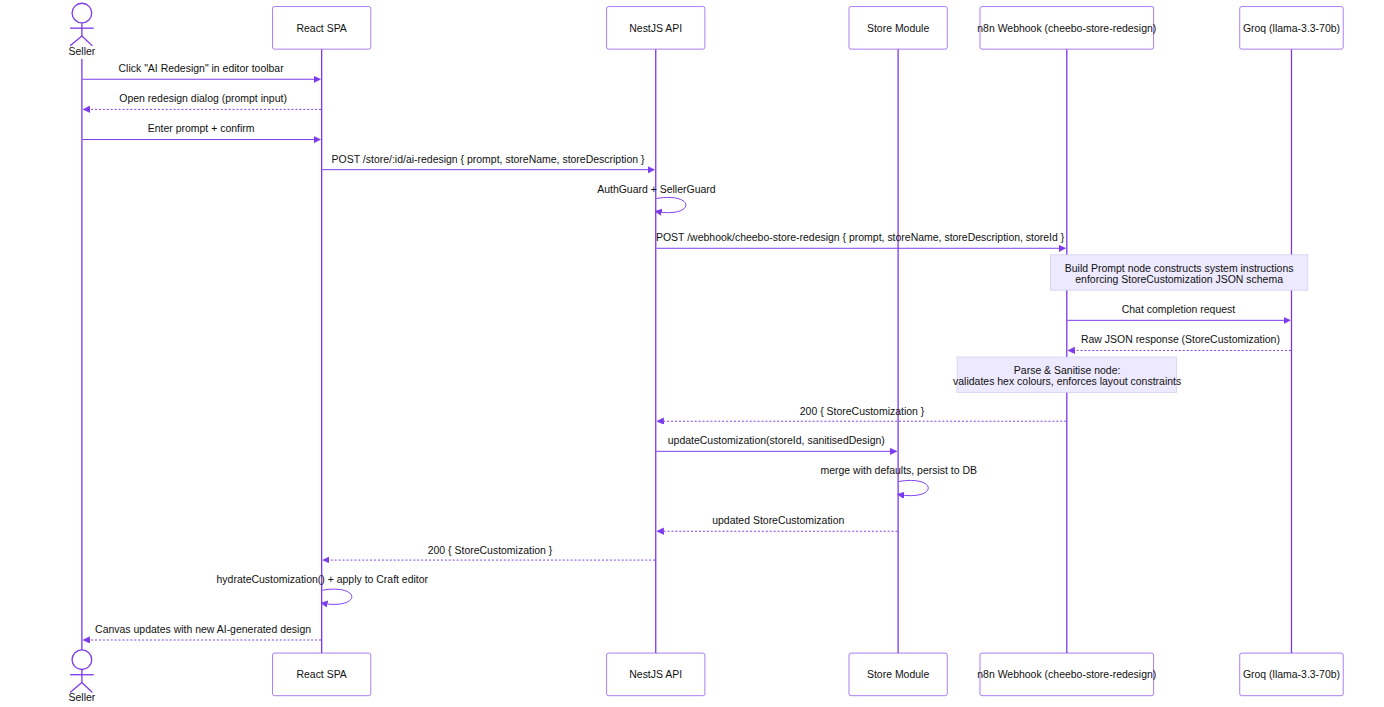
\includegraphics[width=\linewidth]{diagrams/seq-ai-redesign.png}
  \caption{AI storefront redesign --- interaction sequence}
  \label{fig:seq-ai-redesign-design}
\end{figure}

\section{Class Diagram}

Figure~\ref{fig:class-diagram} presents the UML class diagram of
the main domain entities. It highlights the inheritance hierarchy
between \texttt{User}, \texttt{Seller}, and \texttt{Administrator},
the composition relationship between \texttt{Store} and
\texttt{Product}, and the aggregation between \texttt{Order} and
\texttt{OrderItem}.

\begin{figure}[H]
  \centering
  \imagePlaceholder[10cm]{UML class diagram — main domain entities}
  \caption{Class diagram}
  \label{fig:class-diagram}
\end{figure}

% ============================================================
%  CHAPTER 4
% ============================================================
\chapter{Development and Implementation}

\begin{chapterintro}
  This chapter details the development environment, backend and frontend
  implementation decisions, and the AI integration via N8N.
\end{chapterintro}

\section{Development Environment}

\subsection{Hardware and Software}
% TODO

\subsection{VSCode and Extensions}
% TODO

\subsection{pnpm Monorepo Structure}

The project is organised as a \texttt{pnpm} workspace monorepo with
three top-level packages. Figure~\ref{fig:monorepo} shows the
directory tree: \texttt{backend/} contains the NestJS API,
\texttt{frontend/} the React SPA, and \texttt{terraform/} the
infrastructure-as-code definitions.

\begin{figure}[H]
  \centering
  \imagePlaceholder[6cm]{Monorepo directory tree (backend/, frontend/, terraform/)}
  \caption{Cheebo monorepo structure}
  \label{fig:monorepo}
\end{figure}

\section{Backend (NestJS)}

\subsection{Project Structure}
% TODO

\subsection{Key Modules}
% TODO: auth, stores, products, orders, AI

\subsection{Authentication Guards and Role-Based Access Control}

Every protected route is secured through a combination of
\texttt{AuthGuard} and the \texttt{@Roles()} decorator.
Figure~\ref{fig:rbac} shows a representative controller method
annotated with both guards, illustrating how the framework enforces
role-based access at the route level before the handler executes.

\begin{figure}[H]
  \centering
  \imagePlaceholder[5cm]{Code snippet — AuthGuard + @Roles() decorator}
  \caption{Role-based access control implementation}
  \label{fig:rbac}
\end{figure}

\subsection{File Upload System (Multer)}
% TODO

\subsection{Email System (Nodemailer)}
% TODO

\section{Frontend (React + Vite)}

\subsection{Project Structure}
% TODO

\subsection{Routing and Layouts}
% TODO

\subsection{State Management (TanStack Query + Zustand)}
% TODO

\subsection{Admin Dashboard Panels}

Figure~\ref{fig:admin-dashboard} shows the administrator dashboard,
which centralises seller application reviews, store moderation, user
management, and featured content curation in a single tabbed
interface.

\begin{figure}[H]
  \centering
  \imagePlaceholder[8cm]{Screenshot — Admin dashboard}
  \caption{Admin dashboard}
  \label{fig:admin-dashboard}
\end{figure}

\subsection{Store and Product Management Interface}

Figure~\ref{fig:seller-dashboard} presents the seller-facing store
and product management panels, from which a seller can create and
edit their store, manage their product catalogue, upload images,
and monitor incoming orders.

\begin{figure}[H]
  \centering
  \imagePlaceholder[8cm]{Screenshot — Store / product management (seller view)}
  \caption{Store and product management interface}
  \label{fig:seller-dashboard}
\end{figure}

\section{AI Integration with N8N}

\subsection{AI Product/Store Verification Pipeline}
% TODO

\subsection{Database Chat Assistant}
% TODO

\subsection{N8N Workflow --- AI Storefront Redesign}

The AI Storefront Redesign workflow allows a seller to regenerate their
entire store visual identity by providing a short natural-language prompt
from inside the Craft.js editor. The sequence is illustrated in
Figure~\ref{fig:seq-ai-redesign}.

\begin{figure}[H]
  \centering
  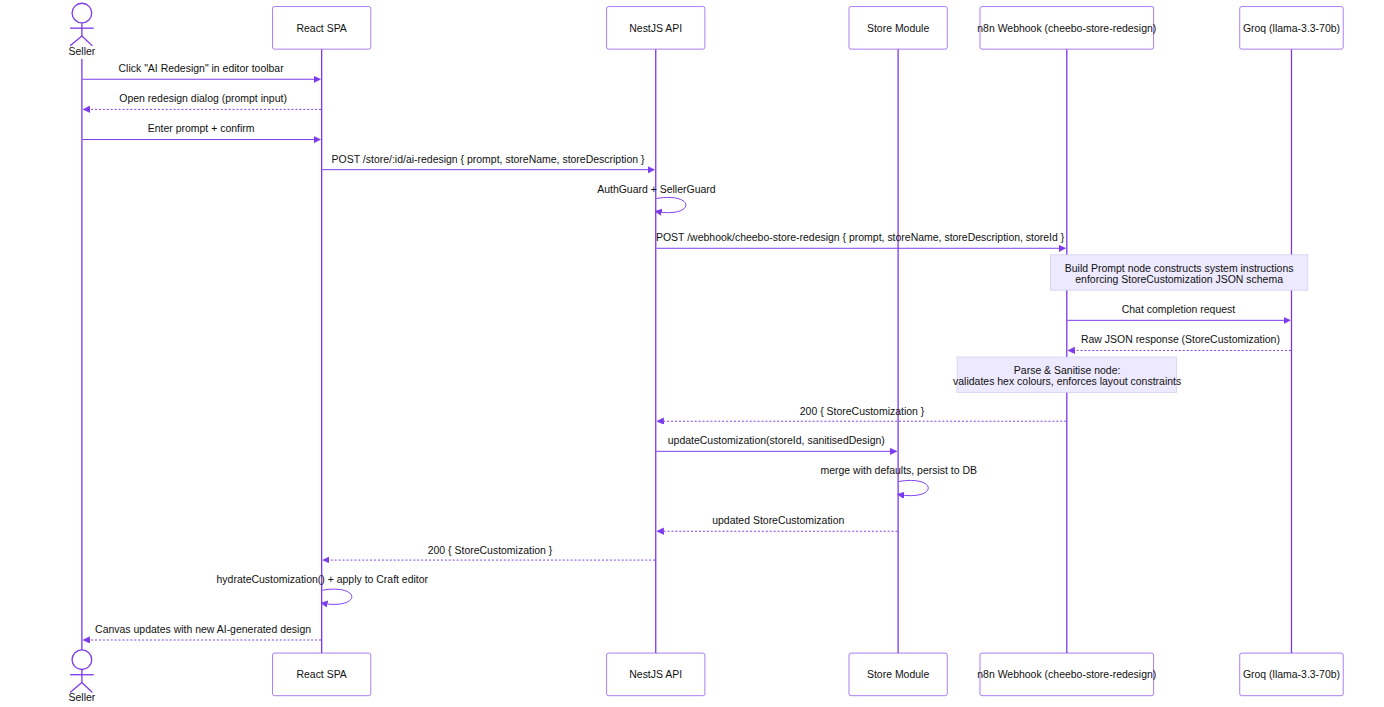
\includegraphics[width=\linewidth]{diagrams/seq-ai-redesign.png}
  \caption{Sequence diagram --- AI storefront redesign workflow}
  \label{fig:seq-ai-redesign}
\end{figure}

The seller clicks the \textit{AI Redesign} button in the editor toolbar,
which opens a dialog prompting for a short description of the desired
aesthetic (e.g.\ \textit{"dark luxury jewellery brand with gold accents"}).
The React frontend calls \texttt{POST /store/:id/ai-redesign}, passing the
prompt alongside the store name and description for context.

On the backend, the NestJS Store Module forwards the request to the
\textbf{cheebo-store-redesign} n8n webhook.
The workflow consists of three nodes:

\begin{enumerate}
  \item \textbf{Build Prompt} --- a Code node that constructs a
        system-level instruction enforcing a strict JSON schema matching
        the \texttt{StoreCustomization} type. The schema covers every
        configurable section: theme colours and fonts, announcement bar,
        banner, header, product grid, sidebar, and footer.

  \item \textbf{AI Agent} --- an AI Agent node connected to the Groq
        \texttt{llama-3.3-70b-versatile} model. The agent receives the
        assembled system prompt and the seller's free-text request, then
        returns a JSON object conforming to the \texttt{StoreCustomization}
        schema.

  \item \textbf{Parse \& Sanitise} --- a Code node that parses the raw
        LLM output, validates all hex colour values with a regex, clamps
        numeric fields to valid ranges, and falls back to safe defaults for
        any field that is missing or malformed.
\end{enumerate}

The sanitised \texttt{StoreCustomization} object is returned to the NestJS
backend, which merges it with the store defaults and persists it through
the existing \texttt{updateCustomization} path. The frontend then calls
\texttt{hydrateCustomization()} on the response and applies the result
directly to the Craft.js editor, giving the seller an immediate live
preview of the AI-generated design without a page reload.

\subsection{Google Gemini / Groq Integration}
% TODO

\subsection{N8N Workflow Implementation}
% TODO

\section{Interface Screenshots}

\subsection{Landing Page}

Figure~\ref{fig:landing} shows the Cheebo public landing page, which
surfaces featured stores, featured products, and the tag-based
recommendation section. The navigation bar provides direct access to
the catalogue, login, and cart.

\begin{figure}[H]
  \centering
  \imagePlaceholder[8cm]{Screenshot — Cheebo landing page}
  \caption{Landing page}
  \label{fig:landing}
\end{figure}

\subsection{Store Dashboard}

Figure~\ref{fig:store-dashboard} presents the seller store dashboard,
from which a seller can monitor live store metrics, access the
customisation editor, and review recent order activity.

\begin{figure}[H]
  \centering
  \imagePlaceholder[8cm]{Screenshot — Seller store dashboard}
  \caption{Store dashboard}
  \label{fig:store-dashboard}
\end{figure}

\subsection{AI Verification Panel}

Figure~\ref{fig:ai-panel} illustrates the AI verification panel
available to administrators. Each entry displays the entity name,
the AI verdict, the LLM rationale, and override controls allowing
the administrator to confirm or reverse the automated decision.

\begin{figure}[H]
  \centering
  \imagePlaceholder[8cm]{Screenshot — AI verification panel (admin)}
  \caption{AI verification panel}
  \label{fig:ai-panel}
\end{figure}

\subsection{Analytics Page}

Figure~\ref{fig:analytics} shows the per-store analytics page
available to sellers, displaying revenue trends, top-selling
products, order volumes, and visitor statistics.

\begin{figure}[H]
  \centering
  \imagePlaceholder[8cm]{Screenshot — Analytics page}
  \caption{Analytics page}
  \label{fig:analytics}
\end{figure}

% ============================================================
%  CHAPTER 5
% ============================================================
\chapter{Infrastructure and Deployment}

\begin{chapterintro}
  This chapter covers Docker containerisation, infrastructure as code with
  Terraform, the GitHub Actions CI/CD pipeline, DNS management, and the
  production environment.
\end{chapterintro}

\section{Containerisation with Docker}

\subsection{Dockerfiles (Frontend and Backend)}
% TODO

\subsection{Docker Compose Configuration}
% TODO

\subsection{Multi-Service Networking}

All services communicate over a private Docker bridge network,
meaning the backend, database, and n8n are never directly exposed
to the public internet. Only the frontend container publishes
port 80. Figure~\ref{fig:docker-network} shows the network topology
and how Nginx on the frontend container proxies all API paths to the
backend service over the internal network.

\begin{figure}[H]
  \centering
  \imagePlaceholder[7cm]{Docker Compose bridge network diagram}
  \caption{Docker Compose network architecture}
  \label{fig:docker-network}
\end{figure}

\section{Infrastructure as Code with Terraform}

\subsection{DigitalOcean Provider}
% TODO

\subsection{VPC, Droplet and Firewall Resources}
% TODO

\subsection{DNS Management with DigitalOcean}

Rather than managing DNS records at the domain registrar (name.com) through a
separate API, the project delegates DNS entirely to DigitalOcean using the same
Terraform provider that manages the droplet.  Two resources are declared in
\texttt{main.tf}:

\begin{itemize}
  \item \texttt{digitalocean\_domain} --- creates the DNS zone for
        \texttt{nadimjebali.engineer} on DigitalOcean's authoritative nameservers
        and automatically adds the apex (\texttt{@}) A record pointing to the
        droplet's IPv4 address.
  \item \texttt{digitalocean\_record} --- adds a second A record for the
        \texttt{www} subdomain, also pointing to the droplet.
\end{itemize}

Both records reference \texttt{digitalocean\_droplet.cheebo.ipv4\_address}
directly.  This means that if the droplet is ever replaced (e.g.\ after a
destructive Terraform change), Terraform updates both DNS records in the same
\texttt{apply} run that creates the new droplet, with no manual intervention
required.

The domain's nameservers are delegated to DigitalOcean
(\texttt{ns1--ns3.digitalocean.com}) from the name.com registrar panel, which
is a one-time configuration step.  After that, A-record updates propagate in
under five minutes thanks to a 300-second TTL.

\begin{keytakeaways}
  \item DNS is version-controlled alongside infrastructure --- the domain
        always points to the current droplet IP with no manual update step.
  \item TTL 300\,s means a full redeploy (destroy old droplet, create new one,
        update DNS) converges in under ten minutes end-to-end.
\end{keytakeaways}

\subsection{Remote State Management with DigitalOcean Spaces}

Terraform state is stored remotely in a DigitalOcean Spaces bucket
configured as an S3-compatible backend. This ensures that every
CI/CD run reads from and writes to a single shared state file,
preventing conflicts if the workflow is triggered concurrently.
Figure~\ref{fig:terraform} shows the key resource declarations in
\texttt{main.tf}, including the VPC, the droplet, and the DNS records.

\begin{figure}[H]
  \centering
  \imagePlaceholder[6cm]{Terraform code snippet --- main.tf}
  \caption{Terraform resources}
  \label{fig:terraform}
\end{figure}

\section{CI/CD Pipeline with GitHub Actions}

\subsection{Workflow Overview}

The CI/CD pipeline is defined as a single GitHub Actions workflow
file that runs on every push to the \texttt{main} branch.
Figure~\ref{fig:cicd} presents the three parallel jobs ---
\textit{provision} (Terraform), \textit{build-backend}, and
\textit{build-frontend} --- followed by the \textit{deploy} job
that SSH-deploys the composed stack once all three complete.

\begin{figure}[H]
  \centering
  \imagePlaceholder[7cm]{CI/CD pipeline diagram (build $\rightarrow$ push $\rightarrow$ deploy)}
  \caption{GitHub Actions CI/CD pipeline}
  \label{fig:cicd}
\end{figure}

\subsection{Build Stage (Docker Build and Push to Docker Hub)}
% TODO

\subsection{Deployment Stage (SSH and Docker Compose)}
% TODO

\subsection{Environment Secrets Management}
% TODO

\section{Production Environment}

\subsection{DigitalOcean Droplet Specifications}

The production workload runs on a single DigitalOcean droplet provisioned by
Terraform with the following specifications:

\begin{center}
\begin{tabular}{ll}
  \toprule
  \textbf{Property} & \textbf{Value} \\
  \midrule
  Region      & Frankfurt (fra1) \\
  Size        & s-2vcpu-2gb (2 vCPUs, 2 GB RAM) \\
  Image       & Ubuntu 24.04 LTS \\
  VPC         & cheebo-vpc (192.168.1.0/24) \\
  Public URL  & \texttt{http://nadimjebali.engineer} \\
  DNS         & Managed by DigitalOcean (Terraform) \\
  \bottomrule
\end{tabular}
\end{center}

The application is accessed exclusively through the domain name
\texttt{nadim\-jabali.engineer}.  The raw droplet IP is reserved for SSH
access by the CI/CD pipeline and is never exposed to end users.  CORS on
the backend is configured with the domain as the single trusted origin, so
any attempt to reach the API directly from the IP is rejected by the
browser's same-origin policy.

\subsection{Production Service Architecture}

Figure~\ref{fig:production} depicts the production environment as
deployed on the DigitalOcean droplet. All four Docker Compose
services run on the same host inside a private bridge network;
only the frontend Nginx container is reachable from the public
internet via the domain \texttt{nadimjebali.engineer}.

\begin{figure}[H]
  \centering
  \imagePlaceholder[7cm]{Production environment diagram (Droplet + services)}
  \caption{Production architecture}
  \label{fig:production}
\end{figure}

\subsection{N8N Deployment Alongside the Application}
% TODO

% ============================================================
%  GENERAL CONCLUSION
% ============================================================
\chapter*{General Conclusion}
\addcontentsline{toc}{chapter}{General Conclusion}
\markboth{General Conclusion}{}

\section*{Summary of Achievements}
% TODO

\section*{Implemented Features vs Initially Planned Features}
% TODO

\section*{Challenges Encountered and Solutions Provided}
% TODO

\section*{Current Implementation Limitations}
% TODO

\section*{Future Improvements}
% TODO: Konnect payment, mobile app, LM Studio local AI, recommendation engine, advanced analytics

% ============================================================
%  BIBLIOGRAPHY
% ============================================================
\newpage
\addcontentsline{toc}{chapter}{Bibliography and Webography}
\chapter*{Bibliography and Webography}

\begin{itemize}
  \item NestJS Official Documentation --- \url{https://docs.nestjs.com}
  \item React Official Documentation --- \url{https://react.dev}
  \item Prisma ORM Documentation --- \url{https://www.prisma.io/docs}
  \item TanStack Query Documentation --- \url{https://tanstack.com/query}
  \item Docker Documentation --- \url{https://docs.docker.com}
  \item Terraform Documentation --- \url{https://developer.hashicorp.com/terraform}
  \item N8N Documentation --- \url{https://docs.n8n.io}
  \item GitHub Actions Documentation --- \url{https://docs.github.com/en/actions}
  \item DigitalOcean Developer Docs --- \url{https://docs.digitalocean.com}
\end{itemize}

% ============================================================
%  APPENDICES
% ============================================================
\appendix

\chapter{Complete Prisma Schema}

\begin{lstlisting}[caption={Prisma schema --- excerpt}]
% TODO: paste the contents of backend/prisma/schema/ here
\end{lstlisting}

\chapter{API Endpoints Reference}

% TODO: full table of all endpoints

\chapter{N8N Workflow JSON Exports}

\begin{lstlisting}[language=,caption={N8N workflow --- AI verification (JSON)}]
% TODO: paste the JSON exported from N8N
\end{lstlisting}

\chapter{Docker Compose File}

\begin{lstlisting}[caption={docker-compose.yml}]
% TODO: paste the contents of docker-compose.yml
\end{lstlisting}

\chapter{GitHub Actions Workflow}

\begin{lstlisting}[caption={.github/workflows/deploy.yml}]
% TODO: paste the CI/CD workflow content
\end{lstlisting}

\end{document}
